\documentclass[10pt]{article}
\usepackage[a4paper,margin=1.8cm]{geometry}
\usepackage[T1]{fontenc}
\usepackage{lmodern}
\usepackage{graphicx}
\usepackage{booktabs}
\usepackage{amsmath,amssymb}
\usepackage{array}
\usepackage{caption}
\usepackage[table]{xcolor}
\usepackage[authoryear,round]{natbib}\usepackage[hidelinks]{hyperref}
\renewcommand{\cite}{\citep}
\usepackage{titling}
\setlength{\droptitle}{-3.2em}\setlength{\thanksmarkwidth}{0pt}
\postdate{\par\end{center}\vspace{-2.4em}}\preauthor{\begin{center}\large\lineskip 0.2em\begin{tabular}[t]{c}}\predate{\begin{center}\large}\postauthor{\end{tabular}\par\end{center}\vspace{-1.2em}}
\captionsetup{font=small,labelfont=bf}
\graphicspath{{figures/}}
\setlength{\emergencystretch}{3em}
\setlength{\bibsep}{0pt}\setlength{\textfloatsep}{10pt plus 2pt minus 2pt}\setlength{\floatsep}{8pt plus 2pt minus 2pt}\setlength{\intextsep}{8pt plus 2pt minus 2pt}
\renewcommand{\floatpagefraction}{0.8}\renewcommand{\topfraction}{0.9}\renewcommand{\bottomfraction}{0.8}\renewcommand{\textfraction}{0.08}
\makeatletter\newcommand{\tightbib}{\footnotesize\def\@listi{\leftmargin\leftmargini\parsep\z@\topsep 2\p@\itemsep\z@}}\makeatother
\newcommand{\ci}[2]{[#1,\,#2]}
\newcommand{\sd}{\textsc{FileInfo}}
% text that depends on analyses still running when this file was last edited renders as a visible red marker
\newcommand{\pending}[1]{\textcolor{red}{\textbf{[PENDING: #1]}}}
\newcommand{\powersyll}{The syllable-level battery (30,000 syllable shapes; Supplement Table~S2b) behaved alike but was somewhat less sensitive: two equally common types were detected in 80--92\% of replicates at 4 standard deviations, a 20\% minority in 83--99\% at 6 (silhouette, prediction strength, Jaccard and dip statistics), and a 5\% minority in at most 9\% of replicates up to 6 standard deviations (dip statistic 64\% at 8).}

\title{Discrete or graded? A confound-controlled re-analysis of clustering\\ in Egyptian fruit bat (\textit{Rousettus aegyptiacus}) social calls}
\author{Ninad Rai\\Ashoka University}
\date{}

\begin{document}
\maketitle
\vspace{-1.3em}

\begin{abstract}
\noindent\textbf{Background.} Unsupervised clustering is used to define animal call types, but clusters can reflect recording conditions rather than call structure. Earlier analyses of a public Egyptian fruit bat corpus reported two acoustic regimes and individual ``acoustic modes''.
\textbf{Methods.} We re-derived both analyses from the audio (41,116 annotated recordings for development, 45,557 further files for out-of-sample tests), controlled for silence, duration, signal-to-noise ratio, microphone channel, session and individual, resampled individuals, and compared fifteen clustering algorithms, tests that allow one cluster with measured power, and UMAP--HDBSCAN against null data.
\textbf{Results.} The original matrix was reproduced exactly once file-name integers were read as annotation-table row indices, which showed that its emitter and context labels belonged to other recordings. The two clusters split short, silent from longer voiced recordings (silence AUC 0.89). On voiced frames fuzzy c-means collapsed to one cluster, prediction strength across individuals was 0.66 and no density valley appeared; the tests detect equal-share types four standard deviations apart, not a 5\% minority. One group was separable: pups' Isolation calls (6--7\% of files), recovered by several algorithms and separable on unseen individuals (AUC 0.98), on held-out channels (0.98) and in 12,000 and 33,557 never-used files (0.988, 0.991). Identity was decodable on unseen days (accuracy 0.56; majority class 0.15) but only weakly across microphones (balanced accuracy 0.125; shuffled 0.036).
\textbf{Conclusions.} Social calls are better described as graded than as two discrete regimes, with one separable Isolation group; claims of call types or individual modes need blocked validation, power estimates and null comparisons.
\end{abstract}
\vspace{-0.6em}

\noindent\textbf{Keywords:} bioacoustics; \emph{Rousettus aegyptiacus}; cluster validation; clusterability; confounding; reproducibility; vocal individuality

\section{Introduction}
Egyptian fruit bats (\emph{Rousettus aegyptiacus}) are social, vocal mammals with a large public annotated call corpus \cite{prat2017} whose calls carry emitter, addressee, context and behaviour information \cite{prat2016}. Whether their acoustic space holds discrete call types or varies continuously matters for describing repertoires: hard clustering handles gradation poorly and fuzzy clustering has been recommended \cite{wadewitz2015,fischer2017}, while latent-space projection with density clustering \cite{sainburg2020,thomas2022} and autoencoder or pretrained embeddings \cite{goffinet2021,best2023,aves2023,stowell2022} are now widely used.

We audit two earlier analyses of this corpus (Section~2). (Q1) Can the original analysis be reproduced, and do its labels belong to its audio? (Q2) Do its clusters follow silence, duration, noise, channel, session or date? (Q3) Is there discrete structure in voiced frames and syllables when one cluster is allowed, individuals are resampled and power is known? (Q4) Does any call group survive validation blocked by individual, channel and session, and replicate in unused recordings? (Q5) How much individual and context information transfers across recording conditions? Out-of-sample criteria were fixed beforehand, and part of the original analysis rested on labels that did not belong to its audio.

\section{Background}
Such analyses are fragile for four reasons. First, fuzzy c-means \cite{bezdek1984} and its validity indices \cite{xiebeni1991,rousseeuw1987} cannot return a single cluster, clusterability tests \cite{adolfsson2019,liu2008} are rarely reported, and low-dimensional maps can mislead \cite{chari2023}. Second, clusters may follow recording properties (silence, background noise, microphone) rather than call structure. Third, calls from one file, individual or session are not independent, so ordinary tests and random splits overstate evidence \cite{hurlbert1984} and generalisation \cite{roberts2017}. Fourth, in colony recordings individuals are confounded with place and time.

Two earlier analyses applied FCM to summary features of this corpus: a June analysis described ``a fluid, continuous manifold'' with individual ``acoustic modes'', and a July manuscript reported two ``reproducible acoustic regimes'' linked to context and emitter.

\section{Methodology}
This section covers data and samples (3.1), features (3.2), clustering algorithms (3.3), single-cluster tests, nulls and power (3.4), the latent-space pipeline, the Isolation group and the out-of-sample criteria (3.5), confound, mixed-model and identity analyses (3.6), and implementation (3.7). Further detail is in Supplement S0.

\subsection{Data}
\paragraph{Dataset A.} The corpus of \citet{prat2017} holds 293,238 mono recordings (16-bit, 250\,kHz) in 30 archives (channel, treatment and timestamp per file in \sd{}\texttt{.csv}) with 91,080 annotations on 87,986 files (emitter, addressee, context, actions, annotated span). Emitter codes (meanings in S0): 39,147 annotations (43\%) carry positive codes (41 bats), 44,075 (48\%) negative codes and 7,858 (9\%) code 0. The annotated span starts at sample 1 in 94\% of rows (median 1.48\,s), so it is nearly the whole recording, only a median 12.6\% of it voiced (authors' segments). Audio was streamed by HTTP range requests and none was kept.

\paragraph{Samples.} The \emph{discovery sample} is 41,116 annotated files, one annotation row each, stratified by channel $\times$ month (77 cells, at least 20 files per cell), with at least 200 files per bat and 500 per context where the corpus allows (18,450 files with positive emitter codes, 19,170 negative, 3,496 code 0; 12 channels, 14 months, 30 archives). All development and test choices were made here; the first 15,992 files agreed with the full set, which we report. Two \emph{out-of-sample sets} came from annotated files not extracted earlier: a \emph{replication sample} of 12,000 files drawn uniformly at random (695 Isolation files) and a \emph{completion sample} of all remaining 33,557 annotated files (2,089 Isolation files), so that every annotated file was analysed once (1,313 further files had been extracted only to reproduce the June table). The other 205,252 recordings are unannotated and unused. Their criteria (Section~3.5) were logged before any of their files was analysed.

\paragraph{Dataset B.} \citet{elie2024} recorded 10 adult bats (5 deaf) simultaneously with an ambient microphone (192\,kHz) and a throat-mounted piezo sensor (50\,kHz): 14,844 events on 13 days, no context labels, 12,417 events valid in both sensors analysed. A non-exhaustive web search found no other public corpus.

\paragraph{Original analyses.} The July manuscript used 3,897 rows (2,360 distinct annotation rows) and FCM with $c=2$ (FPC 0.5786, Xie--Beni 1.2498, silhouette 0.2195, cluster sizes 1,860/2,037); the June analysis used 16,000 rows (10 bats $\times$ 1,600) and a six-test battery. We used the saved arrays of the former and the call-level output of the latter.

\subsection{Features and representations}
\emph{Whole-span (original) features}: a 128-band mel spectrogram (2--125\,kHz, power in decibels; librosa \cite{mcfee2015}), its deltas and seven per-band statistics, 1,408 features over the annotated span. \emph{Voiced-frame features} apply the same statistics to frames inside a voiced segment, with 20 MFCCs and deltas (120 statistics) and per-file recording covariates such as silence fraction and signal-to-noise ratio (SNR; full list in S0). \emph{Syllable features} describe 141,815 voiced segments of at least 3 frames, including a duration- and level-free \emph{shape} of 512 values; 30,000 random segments were analysed. A variational autoencoder \cite{goffinet2021} was trained on the shapes of 21 random bats (16,490 syllables) and applied to the 13,510 syllables of the other 21; AVES embeddings \cite{aves2023} (two models, four variants) were taken for 1,000 files. Features were standardised and reduced to 50 principal components fitted on the analysed set (the discovery set for the out-of-sample sets), and every stochastic step used seed 42 (details in S0).

\subsection{Clustering algorithms}
Fifteen clustering algorithms (26 variants, including fuzzy c-means with $m=2$, tolerance 0.005 and 20, 5 or 3 restarts depending on the analysis (Supplement S0), and HDBSCAN \cite{campello2013}) were run with scikit-learn \cite{pedregosa2011} on 19 representations (Supplement S0), each a seeded 6,000-point subsample (all points for the 1,000-file sets); silhouettes used a 3,000-point subsample. A partition counted as candidate structure only if at least two clusters held at least 1\% of the points (single linkage otherwise ``wins'' with singletons). \emph{Bat-transfer stability} of the best-silhouette configuration of each family was the adjusted Rand index \cite{hubert1985} between a fit on one random half of the bats, transferred (5-nearest neighbours) to the other half, and a fit on that half itself (two splits); on the full discovery sets FCM, k-means, diagonal GMM and HDBSCAN also report held-out-bat stability.

\subsection{Tests that allow a single cluster, nulls and power}
All tests resample \emph{bats}, not calls: the gap statistic \cite{tibshirani2001}; prediction strength \cite{tibshirani2005} at $k=2$ with halves split by bat (20 splits); bootstrap Jaccard stability \cite{hennig2007} (50 bat resamples); and a split-sample Hartigan dip test \cite{hartigan1985} on the axis between two $k$-means centroids learned on half of the bats and applied to the other half. Each statistic was compared with two nulls of 50--100 datasets: a \emph{Gaussian-copula} null (empirical marginals and rank correlations kept) and a \emph{session-mean} null (copula residuals about channel $\times$ month means, means added back). For power, a two-type mixture was spiked into the session-mean null of the voiced file-level features and syllable shapes (6,000 rows): a fraction $\pi\in\{0.5,0.2,0.05\}$ of rows, chosen independently of bat, was shifted by $\delta\in\{1,2,3,4,6,8\}$ standard deviations along a random direction in the top ten components. The battery ran on 200 replicates per cell; a statistic detected the structure when it exceeded the 95th percentile over 200 null replicates (settings and a single-population control in S0).

\subsection{Latent-space pipeline and the Isolation group}
\paragraph{UMAP and HDBSCAN.} The standard bioacoustic pipeline \cite{mcinnes2018,sainburg2020,thomas2022} (UMAP to 10 dimensions, 30 neighbours, minimum distance 0; HDBSCAN minimum cluster size 30, 100 and 300) was run on 12,000 random files: on the real data, on 12 Gaussian-copula and 12 session-mean nulls, on six curved-continuum nulls and three nulls with skewed marginals, on the real data without the resulting small cluster or without all Isolation-context files, and under 8 bat bootstraps and with 15 and 100 neighbours. Clusters were characterised by recording covariates, context and a held-out-bat discriminant axis (S0).

\paragraph{Supervised separability.} A balanced logistic regression predicted Isolation against all other contexts from the 50 components with folds blocked by bat (AUC with bat-level bootstrap intervals, $d'$ and dip tests of the out-of-fold scores). It was repeated within pups only, within channel $\times$ month strata, per pup, without the unknown-emitter group, within pup-age windows, with each channel or treatment held out in turn, and for syllables, the VAE and AVES.

\paragraph{Out-of-sample criteria (fixed beforehand).} A model trained on all discovery files must separate Isolation from other contexts in the new files with AUC $\ge0.90$ (C1); UMAP and HDBSCAN (minimum size 100) fitted on the new files alone (a seeded 12,000-file subsample for the completion sample) must return a cluster of 3--12\% of the files of which at least 70\% are Isolation-context (C2); and six copula nulls must return more clusters and more noise than the real data (C3, a weak criterion given the fragility of these statistics). The negative results were re-tested on the same files: FCM collapse on voiced features, the silence/duration axis of the whole-span label, and the battery against ten copula nulls.

\subsection{Confound audit, mixed models and identity}
The cluster label was related to continuous and categorical covariates (AUC; bias-corrected Cram\'er's $V$ \cite{bergsma2013}) with bat-level bootstrap intervals and tested within channel $\times$ month strata by permutation; recording variables alone predicted it by logistic regression with folds blocked by bat. Mixed models used crossed random intercepts for bat and stratum (statsmodels \cite{seabold2010}). Emitter identification (40 of the 41 positive-coded bats, those with at least 30 files; Supplement Table~S0b) used multinomial logistic regression with random, day-, month-, archive- and channel-blocked folds, balanced accuracy and a permutation null (labels shuffled within channel $\times$ month strata); label-free channel normalisation was tested as a remedy (S0).

\subsection{Implementation and reproducibility}
Code, seeds, package list and the chronological analysis log are in the project repository and in S0. The original feature extraction code was not available.

\section{Results}
\subsection{The original analysis is reproduced exactly; the original labels belong to other files}
Reading the integer in each original file name as a file identifier did not reproduce the saved feature matrix (correlation of the first component 0.10--0.12; ARI against the original labels $\approx0.005$). The integers are instead \emph{row indices} of the annotation table: the June table's emitter column matches \texttt{Annotations.csv} row $n$ in 100.0\% of its 16,000 rows (and the file with identifier $n$ in 0.1\%). With the audio of row $n$ and a per-file-maximum decibel reference, the 1,408-feature matrix and its PCA reproduced the saved array to $|r|=1.000$ for components 1--5; FCM then gave FPC 0.5786, Xie--Beni 1.2496, silhouette 0.2195, cluster sizes 1,860/2,037 and ARI $=1.000$ against the original labels (Supplement Table~S0); other decibel references failed (ARI 0.72 and 0.73), and the original duration contrast was reproduced exactly (medians 1.966\,s vs.\ 1.314\,s, point-biserial $r=-0.4223$ vs.\ $-0.422$).

The original emitter and context arrays had been joined to the audio by file identifier. They agree with the true annotation of the audio in 0.2\% (emitter) and 22.6\% (context) of rows and with the identifier reading in 98.2\%. The published associations of the clusters with context ($V=0.145$) and emitter ($V=0.233$) therefore relate cluster labels from one set of recordings to metadata of another. With the true labels, $V=0.311$ for context (bias-corrected 0.307, bat-level 95\% CI \ci{0.15}{0.43}) and $V=0.441$ for emitter (bias-corrected 0.438, \ci{0.22}{0.56}; only 10 bats occur, not 35 levels); within channel$\times$month strata the context $V$ was 0.299 against a permutation null of 0.235 (0 of 2,000), a modest excess (Supplement, Fig.~S1). The June table has the same problems: its 16,000 ``balanced'' calls are 9,588 distinct annotation rows, its cluster follows the same silence and length axes (AUC 0.887), and its two ``specialist'' bats were recorded in one treatment (Supplement Section~10).

\subsection{The original pipeline clusters recordings by silence and duration}
On 41,116 files, the whole-span FCM partition ($c=2$, FPC 0.583, silhouette 0.229) tracked the silence fraction (AUC 0.887, \ci{0.856}{0.906}), voiced duration (0.905 inverted) and span length (0.844 inverted), not SNR (0.477, \ci{0.448}{0.507}). Silence and length variables alone predicted the label on held-out bats with AUC 0.914 (\ci{0.898}{0.927}), noise floor, SNR and clipping alone 0.836, channel alone 0.585, context alone 0.640 and all recording variables 0.968 (\ci{0.960}{0.974}; Fig.~\ref{fig:conf}). The association with context ($V=0.302$) remained above the channel$\times$month null (0.130), but the label is a duration/silence axis and contexts differ in typical duration. The result replicated in the 12,000 and 33,557 never-used files (Section~\ref{sec:repl}).

\begin{figure}[!t]\centering
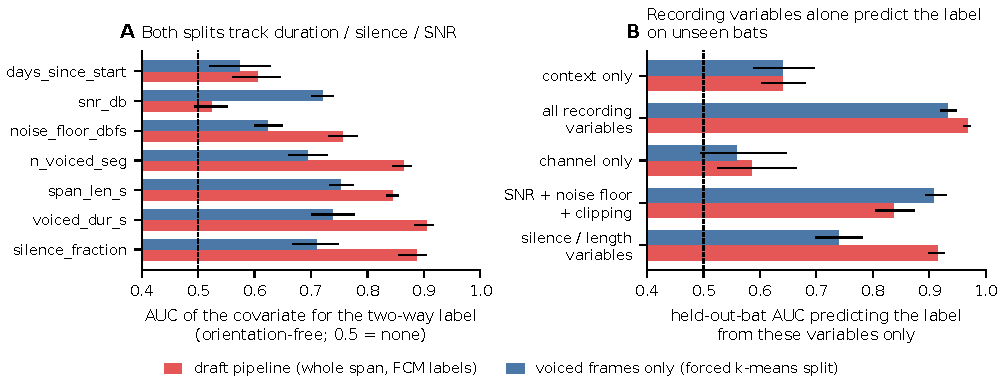
\includegraphics{fig1_v4.pdf}
\caption{(A) AUC of recording covariates for the two-way label from the original whole-span pipeline (red) and from a forced $k$-means split of voiced frames (blue). (B) Held-out-bat AUC when the label is predicted only from the listed variables. Error bars: bat-level 95\% CI.}\label{fig:conf}
\end{figure}

\subsection{Voiced frames: no balanced partition, and what the tests could detect}
With voiced frames only, FCM at $c=2$ gave FPC $=0.5000$ (the one-cluster value) for the 1,408 voiced statistics and for voiced MFCCs; whole-span MFCCs gave 0.511. Simulated single-population data with the original variance spectrum (Gaussian, heavy-tailed, skewed, and a curved one-dimensional continuum; 60 datasets each) gave FPC $\le0.503$ yet ``selected'' $c=2$ by FPC in 100\% of datasets, by silhouette in 77--100\% and by Xie--Beni in 55--63\%, while the real whole-span matrix lay outside this range (FPC 0.579, silhouette 0.220). ``All three indices select $c=2$'' is therefore uninformative: they pick the smallest $c$ tested (Supplement, Fig.~S2).

Tests that allow one cluster and resample bats agreed (Table~\ref{tab:k1}). On the voiced 1,408 statistics, prediction strength across bats was 0.66 (\ci{0.60}{0.85}), below the usual 0.8 rule and below both nulls; bootstrap Jaccard stability was 0.84 against 0.99 and 0.96; the split-sample dip statistic did not clearly exceed the nulls (0.0026 against 0.0024; permutation $p=0.16$ and $0.06$; median dip $p=0.99$, none of 40 splits below 0.05); the gap statistic chose the maximum $k$ for data and nulls alike and is not used. On the original matrix and on the whole-span features re-extracted from 15,992 files, silhouette and FPC exceeded the nulls (an excess that follows duration and SNR, Section~4.2) but prediction strength (0.70, 0.76) and the dip test did not. The silhouette and bootstrap results for voiced MFCCs and 30,000 syllable shapes were alike (Supplement Tables~S1a and S1b).

\begin{table}[!t]\centering\scriptsize
\caption{Clusterability statistics (larger = more cluster-like) against a Gaussian-copula null (cop.) and a session-mean null (ses.); mean of 50--100 null datasets. PS = prediction strength; its bat-level 95\% CI is given in the last row. The full tables for all representations are Supplement Tables~S1a and S1b.}\label{tab:k1}
\begin{tabular}{lccc|ccc|ccc}
\toprule
 & \multicolumn{3}{c|}{original matrix (true bats)} & \multicolumn{3}{c|}{voiced 1,408} & \multicolumn{3}{c}{voiced MFCC} \\
statistic & obs. & cop. & ses. & obs. & cop. & ses. & obs. & cop. & ses. \\
\midrule
FPC$(c{=}2)-0.5$ & 0.079 & 0.041 & 0.026 & 0.000 & 0.000 & 0.000 & 0.000 & 0.000 & 0.000 \\
Silhouette, $c{=}2$ & 0.221 & 0.197 & 0.181 & 0.149 & 0.128 & 0.122 & 0.159 & 0.125 & 0.108 \\
PS, $k{=}2$ & 0.704 & 0.917 & 0.712 & 0.660 & 0.955 & 0.848 & 0.789 & 0.975 & 0.875 \\
Bootstrap Jaccard, $k{=}2$ & 0.875 & 0.971 & 0.892 & 0.845 & 0.986 & 0.956 & 0.955 & 0.994 & 0.965 \\
Split-sample dip & 0.0080 & 0.0087 & 0.0074 & 0.0026 & 0.0024 & 0.0024 & 0.0021 & 0.0021 & 0.0022 \\
\midrule
PS, 95\% CI (bats) & \multicolumn{3}{c|}{\ci{0.62}{0.83}} & \multicolumn{3}{c|}{\ci{0.60}{0.85}} & \multicolumn{3}{c}{\ci{0.74}{0.93}} \\
\bottomrule
\end{tabular}
\end{table}

A negative result is informative only if the same tests would detect a discrete mixture of the same size in the same data. We therefore spiked a two-type mixture into the session-mean null of the voiced features (Fig.~\ref{fig:power}). For two equally common types, prediction strength, silhouette, bootstrap Jaccard stability and the split-sample dip statistic detected the mixture in 90--100\% of replicates at a separation of 4 standard deviations, in 48--70\% at 3 and in at most 15\% at 2. A 20\% minority was detected in 96--100\% of replicates at 6 standard deviations (47--64\% at 4), and a 5\% minority was essentially undetected up to 6 (at most 18\%) and detected only by the dip statistic at 8 (90\%). Equal-weight Gaussian mixtures become bimodal only beyond 2 standard deviations, so the battery is not unusually insensitive; but a negative result excludes well-separated common types, not overlapping, subtle or rare ones. \powersyll

\begin{figure}[!t]\centering
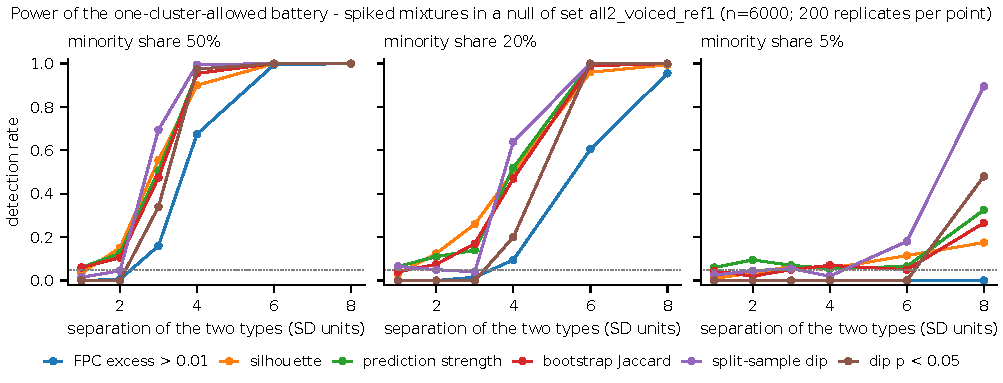
\includegraphics{fig2_v4.pdf}
\caption{Detection rate of the one-cluster-allowed battery for a two-type mixture spiked into a null with no discrete structure (voiced file-level features, 6,000 files, 200 replicates per point). The dotted line is the 5\% false-positive rate. Separation is in standard deviations along a random direction in the top ten principal components.}\label{fig:power}
\end{figure}

\subsection{Fifteen clustering algorithms on nineteen representations}\label{sec:allm}
Because any one algorithm can mislead, we ran fifteen (26 variants, 1,558 configurations) on all 19 representations (Methods; Supplement Fig.~S7, Supplement Table~S7). On the four file-level representations of Dataset A (whole-span and voiced 1,408 statistics, whole-span and voiced MFCC statistics) no algorithm produced a partition that was at once well separated (silhouette $\ge0.25$), stable across bats (transfer ARI $\ge0.6$) and balanced (larger cluster $\le80\%$ of the files). Well-separated, bat-stable partitions did exist, but they were unbalanced and, for voiced features, isolated the Isolation group: spectral clustering of the voiced 1,408 statistics split off a 7\% cluster (silhouette 0.33, transfer ARI 0.91) whose best-matching class was Isolation calls (F1 0.87). Spectral and graph clustering, Ward linkage, BIRCH and tied-covariance mixtures recovered the Isolation group in many representations, whereas fuzzy c-means never did (0 of 17). Admissibility counts, silhouettes, stability and recovery rates for every algorithm are given in Supplement Section~8.



\subsection{Syllables, a learned latent space and pretrained embeddings}\label{sec:syll}
Voiced segments are the natural unit for ``call types''. Across 141,815 syllables (42 emitter groups) the median duration was 85\,ms and the distribution of $\log_{10}$ duration was unimodal (Hartigan dip 0.0012, $p=0.18$; Fig.~S3). Duration alone carried no context information on unseen bats (balanced accuracy 0.066; 13 contexts, chance 0.077), whereas duration-free spectro-temporal shape did (0.198). For 30,000 syllable shapes FCM collapsed (FPC 0.500), prediction strength was 0.73 (\ci{0.68}{0.87}; copula null 0.97) and the other statistics did not exceed the nulls: the file-level result holds for single syllables, with the one exception of Section~\ref{sec:iso}. A variational autoencoder trained on 21 bats and two pretrained AVES models (four variants each) likewise collapsed FCM, showed no structure above the nulls and decoded context no better than handcrafted features (full results in Supplement Section~4).


\subsection{The one separable group: pups' Isolation calls}\label{sec:iso}
This group was found exploratorily in the discovery sample, and the supervised tests below are also exploratory, blocked by bat, channel, treatment and age; the pre-specified validation in held-out files is reported in Section~\ref{sec:repl}.

\paragraph{Exploratory discovery.} The standard UMAP--HDBSCAN pipeline on 12,000 voiced files returned two clusters at minimum sizes 100 and 300, covering 99.6\% of files: a large one (93.2\%) and a small one of 770 files (6.4\%; Fig.~\ref{fig:iso7}A,B). The small cluster was stable under resampling of bats (Jaccard 0.975, range 0.959--0.993 over 8 bootstraps) and under 15 and 100 UMAP neighbours, spanned 30 of 42 emitter groups and several channels (the most common channel held 38\% of it, against 36\% of the large cluster), and was not a duration or silence group (voiced-duration AUC 0.54, silence AUC 0.47; median 1 voiced segment against 2). It was 86\% Isolation-context files (662/770) and contained 83\% of the Isolation files, which are 6.7\% of the sample; among positive-coded pups, 87.8\% of Isolation files fell in the cluster against only 2.0\% of the same pups' files from other contexts and 0.4\% of adults' (non-Isolation) files (NMI 0.651 against a within-channel$\times$month permutation null of 0.062, maximum 0.083; 0 of 1,000). On an axis learned from other bats the two groups were separated by $d'=7.0$ (range 5.7--8.3). Cluster counts and noise shares of HDBSCAN solutions are, however, fragile statistics: null datasets (Gaussian-copula, session-mean, curved-continuum, skewed) fragmented into 2--13 clusters with 38--77\% noise, but the real data with the small cluster removed also fragmented (15 clusters, 48\% noise at minimum size 100, three at size 30; Fig.~\ref{fig:iso7}B), so we do not treat the contrast with the nulls as evidence by itself. Blind recovery was also representation-dependent: on the whole-span features four clusters resulted, one of which (675 files) was 91\% Isolation-context with 77\% of the Isolation files, the others following recording channel (Cram\'er's $V$ of the partition with channel 0.64); on syllable shapes a 464-syllable cluster (3.9\%) was 78\% Isolation-context (82\% of Isolation syllables); on voiced MFCC statistics only a 0.9\% single-channel micro-cluster appeared. The evidence for the group therefore rests on the tests that follow and on the algorithm comparison above, not on the unsupervised discovery alone.

\begin{figure}[!t]\centering
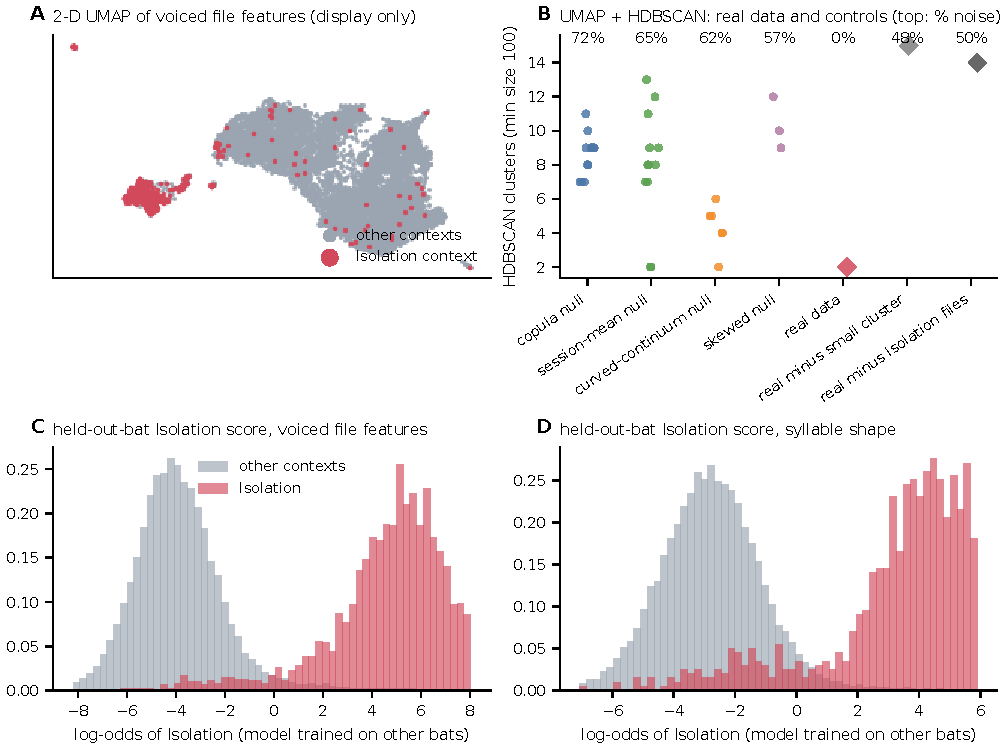
\includegraphics{fig4_v4.pdf}
\caption{(A) 2-D UMAP of 12,000 voiced file feature vectors with Isolation-context files highlighted (display only). (B) Number of HDBSCAN clusters (minimum size 100) for the real data, null datasets without discrete structure (12 Gaussian-copula, 12 session-mean, 6 curved-continuum, 3 skewed) and the real data with the small cluster or all Isolation files removed; the number above each group is the mean share of points labelled noise. (C, D) Held-out-bat score (log-odds of Isolation from a model trained on other bats) for voiced file features (C) and syllable shapes (D).}\label{fig:iso7}
\end{figure}

\paragraph{Supervised separability (discovery sample).} Predicting Isolation from the voiced features with folds blocked by bat gave AUC 0.984 (95\% CI \ci{0.979}{0.991}; voiced MFCCs 0.984), $d'=4.5$, with only 3.2\% of non-Isolation files scoring above the 5th percentile of Isolation files. The pooled out-of-fold score was bimodal (dip $p=3\times10^{-4}$) while the scores of non-Isolation files alone were unimodal ($p=0.996$): the Isolation files formed a separate mode, not the tail of the others (Fig.~\ref{fig:iso7}C). The result held within pups only (AUC 0.982, \ci{0.969}{0.990}; the same 20 pups' other contexts), within channel$\times$month strata (weighted mean 0.90), without the unknown-emitter group that supplies 57\% of Isolation files (0.984), for each of 15 identified pups from a model blind to that pup (median 0.97, range 0.83--1.00), with each channel or treatment held out in turn (0.983 over 8 channels; 0.986 over 6 treatments) and within pup-age windows from day 40 (0.70 at 40--60 days, 0.93 at 60--90, 0.97 at 90--150), although pups younger than 40 days contribute almost only Isolation files (183 against 4), so age and context cannot be separated there. At the syllable level the separation was weaker but clear (AUC 0.956, \ci{0.944}{0.974}; $d'=3.7$; 30--33\% of non-Isolation syllables scored above the 5th percentile of Isolation; Fig.~\ref{fig:iso7}D), and AVES embeddings separated the group no better than handcrafted features (AUC 0.93--0.95 against 0.94--0.97 on 1,000 files). All variants are in Supplement Table~S4; the unsupervised tests could not be expected to find a group this small (Fig.~\ref{fig:power}), and a forced two-way split of all files is dominated by other variation.

\subsection{Pre-specified validation in every remaining annotated file}\label{sec:repl}
Criteria for the two out-of-sample sets were written to the analysis log before any of their files was analysed, and no analysis choice used these files. They come from the same corpus and share all of their positive-coded bats and channels with the discovery sample (Supplement Table~S5b), so they test over-fitting to the discovery recordings, not generalisation to other colonies. All three criteria were met in both sets (Supplement Table~S5; Supplement Fig.~S6b). In the 12,000-file replication sample the model trained on the discovery files separated Isolation from all other contexts with AUC 0.988 (\ci{0.978}{0.992}; $d'=5.1$; pups only 0.985), and UMAP--HDBSCAN fitted on the new files alone returned two clusters (94.2\% and 5.8\%; no noise) of which the small one held 695 files from 24 emitter groups and was 90.1\% Isolation-context. In the completion sample (all 33,557 remaining annotated files; 2,089 Isolation files) the discovery-trained model gave AUC 0.991 (\ci{0.983}{0.995}; $d'=5.1$; pups only 0.989), and UMAP--HDBSCAN on a seeded 12,000-file subsample returned two clusters (93.9\% and 5.6\% of files; 0.45\% noise) of which the small one held 673 files from 26 emitter groups and was 91.5\% Isolation-context. The copula nulls of both samples fragmented into 7--10 clusters with 64--74\% of points labelled noise at minimum size 100 (real data: two clusters, at most 0.45\% noise; Supplement Section~6).


The negative results replicated as well. In the 12,000 unseen files and in the 12,000-file subsample of the completion sample the whole-span (original) features gave FCM FPC 0.586 and 0.587 (discovery 0.583), with the two-way label tracking silence fraction (AUC 0.899 and 0.903; discovery 0.887), voiced duration (0.915, 0.916) and span length (0.842, 0.842); the voiced features gave FPC $=0.5000$, prediction strength across bats 0.70 and 0.66 against 0.95 and 0.955 for the nulls, bootstrap Jaccard stability 0.88 against 0.99, and a split-sample dip statistic of 0.0027 and 0.0028 against 0.0030 (median dip $p=0.996$ and 0.995).

\subsection{Identity is decodable within a microphone but transfers only weakly across microphones}
Emitter identification (40 bats with positive codes; majority class 0.145, chance 0.025) with voiced features reached 0.593 (\ci{0.572}{0.618}) with random splits and 0.560 blocked by day, but 0.202 (\ci{0.115}{0.255}) when entire channels were held out (month 0.487, archive 0.504; Fig.~\ref{fig:id}). Raw accuracy is a poor yardstick for held-out channels, because predictions depend on class frequencies: balanced accuracy was 0.125 against 0.036 when emitter labels were shuffled within channel$\times$month strata (chance 0.025), so cross-channel identity information is present but weak. Normalising channels, as in earlier supervised work \cite{prat2016}, did not rescue the transfer: per-channel mean subtraction, per-channel standardisation and per-channel$\times$month subtraction gave channel-blocked balanced accuracies of 0.099, 0.088 and 0.083 (nulls 0.021, 0.017, 0.006), with the same pattern for whole-span features and syllable shapes (Supplement Table~S3). Channel itself was decodable on unseen bats (accuracy 0.63--0.85, majority 0.36). Within one channel on unseen days, however, identity was recoverable: pooled over 70 bat--channel classes accuracy was 0.648 against a within-channel majority rate of 0.326 ($+0.322$, \ci{0.288}{0.347}). For 16,663 pair-coded files, an identifier trained on positive-coded files assigned a mean probability of 0.461 to the two recognised participants (stratum-shuffle null 0.290; 0 of 100 reached it) and ranked a participant first in 58.7\% of files (null 33.1\%); trained only on other channels, 0.183 against 0.126.

\begin{figure}[!t]\centering
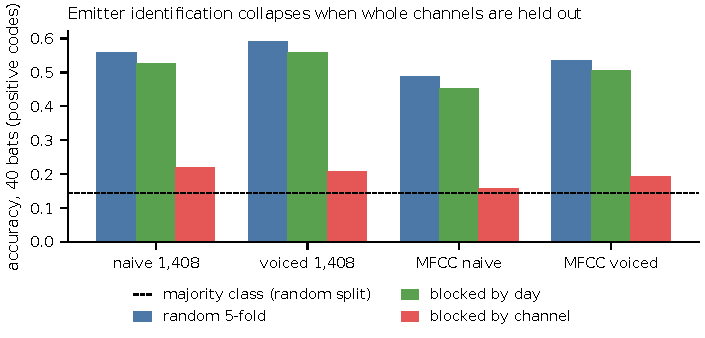
\includegraphics{fig6_v4.pdf}
\caption{Emitter identification from four representations with random, day-blocked and channel-blocked folds (41,116-file discovery sample; horizontal line: majority-class rate).}\label{fig:id}
\end{figure}

\subsection{Context, repeatability and a second dataset}
In mixed models with random intercepts for bat and channel$\times$month stratum, context remained significant for the whole-span label (likelihood-ratio $\chi^2=1{,}643$, df 12; 315 among positive-coded bats) and for a forced voiced split ($\chi^2=1{,}485$ and 366; all $p<10^{-16}$); repeatability by bat was 0.075 (\ci{0.058}{0.109}) for the whole-span label and 0.132 (\ci{0.095}{0.187}) for the voiced split. Context effects were modest (among positive-coded bats, Fighting versus General $-0.45$ logit, \ci{-0.55}{-0.35}, whole-span; Isolation versus General $+0.36$, \ci{0.31}{0.42}, voiced).

In Dataset B the microphone's FCM split (FPC 0.629) followed voiced duration (AUC 0.89) and SNR (0.90), and partitions from the microphone and the piezo agreed beyond chance for the 1,408-statistic features (ARI 0.36--0.44 at $k=2$; shuffled-pairing null 0.00) but largely not within microphone-duration quintiles (ARI 0.02--0.35), i.e.\ the shared structure is event length and loudness. The one-cluster battery gave prediction strength 0.67 (\ci{0.66}{0.85}; nulls 0.97, 0.96) for the microphone, in line with Dataset A. The piezo's two-way split, by contrast, was reproducible across individuals (prediction strength 0.93, \ci{0.82}{0.95}; nulls 0.99, 0.97) and its dip statistic exceeded the session-mean null; it was an event-length and SNR axis, and event length itself is multimodal in Dataset B (Hartigan dip of $\log_{10}$ voiced duration 0.015 and 0.012, $p<10^{-4}$) whereas SNR is unimodal. Because the dataset's authors delimited the events with their detection pipeline, we cannot tell whether this multimodality is behavioural (isolated syllables versus sequences) or procedural. Hearing status and sex were not decodable on held-out individuals (accuracy 0.44--0.59, below the majority rate).

\section{Discussion}
\paragraph{Answer.} Once recording confounds are controlled, Egyptian fruit bat social calls in this corpus are better described as graded than as two discrete regimes, with one exception. The original two clusters split recordings by silence and duration; on voiced frames and syllables, fuzzy and $k$-means clusterings are not reproducible across bats, show no density valley along their axes, and syllable duration is a smooth unimodal continuum. The exception is a group of pups' Isolation-context calls (6--7\% of files). It is recovered blindly by several clustering algorithms (Section~\ref{sec:allm}), generalises across bats and separates from the same pups' calls in other contexts (AUC 0.98 on unseen bats), survives comparison within channel$\times$month strata, with each channel or treatment held out and within pup-age windows from day 40, is a separate mode of the held-out score rather than the tail of the other calls, and replicated, with criteria fixed in advance, in 45,557 annotated files never used before. Linear and fuzzy methods missed it because their tests have little power for a 5--7\% minority (Fig.~\ref{fig:power}) and a two-way split of all files is dominated by silence and duration. We describe it as a separable group of calls that survives bat-, session- and channel-controlled checks, not as a proven call type: Isolation is also a recording situation, and only playback or within-situation contrasts could separate the calls' acoustic distinctness from that of the setting. The only other multimodal quantity, the \emph{length} of the events in Dataset B, may be procedural.

\paragraph{Why the original conclusion arose.} Whole-span features are dominated by silence (a median of 87\% of the annotated span is unvoiced), so validity indices that cannot select one cluster return $c=2$, and an FPC above the collapse value reflects non-Gaussian structure explained by duration. Separately, the original labels were attached to different recordings than the audio that was clustered; checking that a label-independent property (here, duration) agrees between the two sources would have detected this. The original duration contrast reproduced exactly, so descriptors and clusters were consistent and only emitter and context did not belong to them; without the original code we cannot determine how the shift arose.

\paragraph{The answer depends on the algorithm and on the number of clusters allowed.} Fifteen clustering algorithms disagree about how many groups exist, but on the four file-level Dataset A representations none produced a partition that was at once well separated, stable across bats and balanced (Section~\ref{sec:allm}). The algorithms that return a small group (spectral and graph clustering, Ward linkage, BIRCH, tied-covariance mixtures) return the Isolation group; fuzzy c-means never does, and $k$-means does so only when allowed up to six clusters (7 of 17 representations), otherwise returning low-silhouette partitions (median 0.17) that are moderately stable across bats and weakly associated with silence (median NMI 0.12). A single index or algorithm would therefore have misled in either direction: ``two clusters'' from fuzzy c-means on whole-span features, ``no structure'' from fuzzy c-means or $k$-means on voiced features, and ``a small distinct group'' from spectral clustering. Fuzzy c-means collapses on standardised voiced features with at least 20 components but not with 5--10 components or without standardisation, where it again splits on silence and duration (Supplement).

\paragraph{Individuality and place.} Identity is decodable within a microphone on unseen days (0.65 against 0.33) but transfers only weakly across microphones (balanced accuracy 0.125 against a permutation null of 0.036 and 0.46 with random splits), and normalising channels did not help. Bats lived in particular chambers recorded by particular microphones for months, so voice and position are confounded; claims of individual ``acoustic modes'' therefore require recordings of the same individuals on several microphones or in several places. The earlier supervised study reported emitter accuracies of 71\% and 56\% \cite{prat2016}; as we read its Methods they do not describe validation blocked by day, session or channel, so they compare best with our random-split values; we did not re-run that classifier.

\paragraph{Recommendations.} (i) Report FPC minus $1/c$ and never treat ``$c=2$ is optimal'' as evidence for two clusters; test one cluster explicitly. (ii) Compute features on the signal of interest (voiced frames, syllables) and report silence, SNR and duration as covariates. (iii) Resample individuals, never calls, and use channel- and session-blocked evaluation. (iv) When joining labels to features, check an independent property of the recording between sources. (v) Equalise group sizes by subsampling without replacement, and report permutation $p$ as $p<1/(B+1)$. (vi) Treat a battery of tests built from one contingency table as one test. (vii) Measure the power of clusterability tests with spiked mixtures before reading a negative result as absence; run latent-space pipelines against null datasets and with the candidate group removed; treat cluster counts and noise shares as fragile; and confirm any candidate group with a supervised test blocked by individual, channel and session and, if possible, in files never used before.

\paragraph{Limitations.} Only 41 bats have positive emitter codes, 48\% of annotations are pair-coded and 9\% unknown. A negative result does not rule out structure visible to other methods, and recovery of the Isolation group depended on the representation (not found in voiced MFCC statistics by UMAP--HDBSCAN); the tests have little power for minorities below 10\%, and the power analysis used one random direction per replicate with spikes independent of bat. Many analyses were exploratory and the Isolation group emerged post hoc from the UMAP--HDBSCAN run; the supervised tests and both out-of-sample sets confirm it, but share the corpus, bats and recording set-ups and so do not test generalisation to other colonies. Pup age and Isolation are confounded below 40 days, and HDBSCAN cluster counts and noise shares were fragile and are not evidence. The voiced segments come from the dataset authors' segmentation; Dataset B has no context labels, its sensors differ, and its detector threshold is a judgement call. The pretrained-embedding comparison used 1,000 files and the VAE was one small architecture. The original extraction code was not available, so the cause of the label shift is unknown.

\paragraph{Conclusion.} The evidence supports a graded description of Egyptian fruit bat social calls with one separable group of pups' Isolation calls, not two discrete regimes, and shows how routine practice --- clustering whole recordings, trusting validity indices that cannot choose one cluster, and validating with random splits --- can produce a convincing but wrong picture. Whether the Isolation group is a call type, and how much of individual identity is voice rather than position, require new recordings rather than new algorithms.

\sloppy \paragraph*{Author contributions.} N.R. conceived the study, performed the analysis and wrote the manuscript.

\paragraph*{Disclosure statement.} The author declares no competing interests.

\paragraph*{Funding.} This research received no specific funding.

\paragraph*{Data availability statement.} Source data are public (\citet{prat2017}: Figshare collection doi:10.6084/m9.figshare.c.3666502; \citet{elie2024}: doi:10.6084/m9.figshare.25886023). Code, result tables, figures, supplementary data files SD1--SD7 and the chronological analysis log are in the public repository \url{https://github.com/NapolianAdmin/fruit-bat-call-clustering-audit} (doi:10.5281/zenodo.23662435); the compact per-file features (no audio) are available from the author. All steps run from scripts with fixed seeds.

\paragraph*{Ethics and use of AI assistance.} This study re-analysed public recordings; the animal work belongs to the original studies. The analysis code, numerical re-analysis and first draft were produced with an AI coding assistant (Claude Code) on the author's data and instructions; all numbers trace to the scripts and analysis log, and the author is responsible for verifying them.

\begingroup\tightbib
\begin{thebibliography}{xxxxxxxxxxxxxxxxxxxxxxxxxxxxxxxx}\small
\bibitem[Adolfsson et~al.(2019)]{adolfsson2019} Adolfsson A, Ackerman M, Brownstein NC (2019). To cluster, or not to cluster: an analysis of clusterability methods. \emph{Pattern Recognition}. 88:13--26. doi:10.1016/j.patcog.2018.10.026
\bibitem[Bergsma(2013)]{bergsma2013} Bergsma W (2013). A bias-correction for Cram\'er's V and Tschuprow's T. \emph{J Korean Stat Soc}. 42:323--328.
\bibitem[Best et~al.(2023)]{best2023} Best P, Paris S, Glotin H, Marxer R (2023). Deep audio embeddings for vocalisation clustering. \emph{PLoS ONE}. 18(7):e0283396. doi:10.1371/journal.pone.0283396
\bibitem[Bezdek et~al.(1984)]{bezdek1984} Bezdek JC, Ehrlich R, Full W (1984). FCM: The fuzzy c-means clustering algorithm. \emph{Computers \& Geosciences}. 10(2--3):191--203.
\bibitem[Campello et~al.(2013)]{campello2013} Campello RJGB, Moulavi D, Sander J (2013). Density-based clustering based on hierarchical density estimates. \emph{PAKDD 2013, LNCS}. 7819:160--172. doi:10.1007/978-3-642-37456-2\_14
\bibitem[Chari and Pachter(2023)]{chari2023} Chari T, Pachter L (2023). The specious art of single-cell genomics. \emph{PLoS Comput Biol}. 19(8):e1011288. doi:10.1371/journal.pcbi.1011288
\bibitem[Elie et~al.(2024)]{elie2024} Elie JE, Muroy SE, Genzel D, et al. (2024). Role of auditory feedback for vocal production learning in the Egyptian fruit bat. \emph{Current Biology}. 34(17):4062--4070.e7. doi:10.1016/j.cub.2024.07.053 (data: doi:10.6084/m9.figshare.25886023).
\bibitem[Fischer et~al.(2017)]{fischer2017} Fischer J, Wadewitz P, Hammerschmidt K (2017). Structural variability and communicative complexity in acoustic communication. \emph{Animal Behaviour}. 134:229--237. doi:10.1016/j.anbehav.2016.06.012
\bibitem[Goffinet et~al.(2021)]{goffinet2021} Goffinet J, Brudner S, Mooney R, Pearson J (2021). Low-dimensional learned feature spaces quantify individual and group differences in vocal repertoires. \emph{eLife}. 10:e67855. doi:10.7554/eLife.67855
\bibitem[Hagiwara(2023)]{aves2023} Hagiwara M (2023). AVES: Animal Vocalization Encoder Based on Self-Supervision. In: \emph{ICASSP 2023 -- IEEE International Conference on Acoustics, Speech and Signal Processing}. 1--5. doi:10.1109/ICASSP49357.2023.10095642; arXiv:2210.14493.
\bibitem[Hartigan and Hartigan(1985)]{hartigan1985} Hartigan JA, Hartigan PM (1985). The dip test of unimodality. \emph{Ann Statist}. 13(1):70--84.
\bibitem[Hennig(2007)]{hennig2007} Hennig C (2007). Cluster-wise assessment of cluster stability. \emph{Comput Stat Data Anal}. 52(1):258--271.
\bibitem[Hubert and Arabie(1985)]{hubert1985} Hubert L, Arabie P (1985). Comparing partitions. \emph{J Classification}. 2:193--218.
\bibitem[Hurlbert(1984)]{hurlbert1984} Hurlbert SH (1984). Pseudoreplication and the design of ecological field experiments. \emph{Ecol Monogr}. 54(2):187--211.
\bibitem[Liu et~al.(2008)]{liu2008} Liu Y, Hayes DN, Nobel A, Marron JS (2008). Statistical significance of clustering for high-dimension, low-sample size data. \emph{J Am Stat Assoc}. 103(483):1281--1293.
\bibitem[McFee et~al.(2015)]{mcfee2015} McFee B, et al. (2015). librosa: Audio and music signal analysis in Python. \emph{Proc 14th Python in Science Conf}. 18--25.
\bibitem[McInnes et~al.(2018)]{mcinnes2018} McInnes L, Healy J, Melville J (2018). UMAP: Uniform Manifold Approximation and Projection for dimension reduction. arXiv:1802.03426.
\bibitem[Pedregosa et~al.(2011)]{pedregosa2011} Pedregosa F, et al. (2011). Scikit-learn: Machine learning in Python. \emph{J Mach Learn Res}. 12:2825--2830.
\bibitem[Prat et~al.(2016)]{prat2016} Prat Y, Taub M, Yovel Y (2016). Everyday bat vocalizations contain information about emitter, addressee, context, and behavior. \emph{Scientific Reports}. 6:39419. doi:10.1038/srep39419
\bibitem[Prat et~al.(2017)]{prat2017} Prat Y, Taub M, Pratt E, Yovel Y (2017). An annotated dataset of Egyptian fruit bat vocalizations across varying contexts and during vocal ontogeny. \emph{Scientific Data}. 4:170143. doi:10.1038/sdata.2017.143
\bibitem[Roberts et~al.(2017)]{roberts2017} Roberts DR, et al. (2017). Cross-validation strategies for data with temporal, spatial, hierarchical, or phylogenetic structure. \emph{Ecography}. 40(8):913--929. doi:10.1111/ecog.02881
\bibitem[Rousseeuw(1987)]{rousseeuw1987} Rousseeuw PJ (1987). Silhouettes: a graphical aid to the interpretation and validation of cluster analysis. \emph{J Comput Appl Math}. 20:53--65.
\bibitem[Sainburg et~al.(2020)]{sainburg2020} Sainburg T, Thielk M, Gentner TQ (2020). Finding, visualizing, and quantifying latent structure across diverse animal vocal repertoires. \emph{PLoS Comput Biol}. 16(10):e1008228. doi:10.1371/journal.pcbi.1008228
\bibitem[Seabold and Perktold(2010)]{seabold2010} Seabold S, Perktold J (2010). statsmodels: Econometric and statistical modeling with Python. \emph{Proc 9th Python in Science Conf}. doi:10.25080/Majora-92bf1922-011
\bibitem[Stowell(2022)]{stowell2022} Stowell D (2022). Computational bioacoustics with deep learning: a review and roadmap. \emph{PeerJ}. 10:e13152. doi:10.7717/peerj.13152
\bibitem[Thomas et~al.(2022)]{thomas2022} Thomas M, Jensen FH, Averly B, et al. (2022). A practical guide for generating unsupervised, spectrogram-based latent space representations of animal vocalizations. \emph{J Anim Ecol}. 91(8):1567--1581. doi:10.1111/1365-2656.13754
\bibitem[Tibshirani and Walther(2005)]{tibshirani2005} Tibshirani R, Walther G (2005). Cluster validation by prediction strength. \emph{J Comput Graph Stat}. 14(3):511--528.
\bibitem[Tibshirani et~al.(2001)]{tibshirani2001} Tibshirani R, Walther G, Hastie T (2001). Estimating the number of clusters in a data set via the gap statistic. \emph{J R Stat Soc B}. 63(2):411--423.
\bibitem[Wadewitz et~al.(2015)]{wadewitz2015} Wadewitz P, Hammerschmidt K, Battaglia D, Witt A, Wolf F, Fischer J (2015). Characterizing vocal repertoires --- hard vs.\ soft classification approaches. \emph{PLoS ONE}. 10(4):e0125785. doi:10.1371/journal.pone.0125785
\bibitem[Xie and Beni(1991)]{xiebeni1991} Xie XL, Beni G (1991). A validity measure for fuzzy clustering. \emph{IEEE Trans Pattern Anal Mach Intell}. 13(8):841--847.
\end{thebibliography}

\endgroup

\end{document}
